\chapter{Evaluation} \label{C:evaluation}

\section{Method}
The primary goal of the project is the minimisation of the time between receiving source code and completing the program's execution. The initial phases including parsing and optimisation can be understood as compile time, while the actual execution phase is equivalent to run time. The goal of the project attempts
to minimised the combined compile time and runtime. 
As the goal of the project is the minimisation of 


In order to evaluate the performance of the project's implementation, its performance is measured on a suite of hopefully representative programs. The scope of potential programs is limited due to the nature of the language. It does not provide many of the useful abstractions common in other languages such as first-class support for numbers and operations such as arithmetic. This makes writing example programs difficult. However, an decent attempt was made at writing programs that would be hypothetically be representative of a typical Kihi program.

Although, in this context, it is difficult to ascertain what properties exactly a hypothetical typical Kihi program would have. The language is completely unsuited to solving practical problems so any program written in must essentially be trivial and impractical. However, the approach taken in the development of this benchmark suite is an attempt at providing significant coverage of potential programs structures. In particular, attacking classes of programs such as those that utilise church numerals, church lists, binding. These features force particular structures to appear within the program. Whether these structures are common or indicative of Kihi as a whole is difficult to ascertain.

However, due to the minimal nature of the Kihi language, that is the fact it only has five operators, means these programs can be analysed from a mechanical perspective rather simply. A basic analysis is shown below which compares the frequency of evaluated instructions.

However, it is then worthwhile to breakdown and understand the performance of each instruction on a deeper technical level. Perhaps the easiest of the instructions to analyse in this manner is drop. Drop simply receives and discards an argument. Discarding an element only requires freeing the memory it occupies which can be understood as a single instruction. 

A large breadth of benchmark programs would have been ideal but due to the limited expressivenes of the language, qualitiatively different benchmark programs were difficult to construct. Ultimately, these programs were sourced from the examples provided in the Kihi web evaluator and in some cases modified for suitability.

Theses results show that the optimisation strategy has a clear positive effect on runtime performance. Although there is a very minor compile time penalty. This is largely due to the fact the the compile time penalty only scales with the size of the program as opposes to its complexity. This is an amazing time complexity trade off. However, the proposed additional algorithms could involve much more complex optimisers.

Additional, the experimental JIT optimisation process is significantly deterimentally effected by this type of scaling. The size of the program increases significantly during run time. This makes the optimisation process much more expensive to do on an ongoing basis.

\todo[inline]{Future work could involve improving this performance. In particular perhaps values can be ignored in the optimisation process?}


The compile time process is independent of program runtime complexity. Instead, the process scales linearly with program
length and depth (that is the depth of the abstractions it contains). The Kihi Runner provides two implementations of the Symbol Detection algorithm, the first was described earlier in section \ref{sec}\todo[inline]{do this ref} and the second is simply a modification of that same algorithm but with restricted depth. This was a somewhat adhoc solution to the poor JIT optimisation performance due to excessive nesting and lack of meaningful abstractions. See count program.

Future work could potentially involve developing an representation capable of encoding these types of deeply nested structures. A simple solution could be to extend the current abstraction implementation with an integer tag to represent the number of parenthesis surrounding the inner program. This would provide a very efficient representation, and would also be relatively simple to detect such structures since the form of the structure is very limited.

This optimisation algorithm ultimately arose from two features found in the previous implementation. The stack executor and the arity analysis. This was an evolution of the symbolic execution found in the arity analyser of older implementations. Whilst this was able to optimise a small subset of programs the benefits were small. The only benefits it provided was due to its ability to detect subprograms that would result in no output,such programs have no effect on the execution so they could simply be discarded, likely reducing the execution time. However, the benefits of this optimisation were neglible. This mechanism was tested on the count program shown before, and there was essentially no effect. This is unsurprising since as the distribution in figure \ref{fig:count_instruction_distribution} shows drop is never executed in that program and thus there would be no chases subprograms that take an input and don't send output. This suggests that benchmarking this strategy on the \todo[inline]{blah program} would have been better as it would have potentially found optimisation symbols of such a nature.

However, regardless, this mechanism was essentially obseleted by the optimiser present in the current implementation which is capable of representing the same essential idea and more. It is able to equally efficiently encode no ops and also programs with outputs.

The results of the preliminary implementation were misrepresentative of the actual performance. This was cause by a IO bottleneck in the implementation. This explains the nearly identical performance of the reduce executor and the stack executor in context of the theoretical performance. It is then evident that the stack executor is much faster of execution than the reduce executor. However, regardless both executors are still interesting research subjects and the optimisation techniques are applicable to both impementations.

However as the figures show the effect of the optimisations are significantly reduced/larger/essentially the same as the effect of the optimisations on the stack executor.

Looking at the results of the optimisations it is clear that optimisation level one provides a significant boost to the performance of the reduce executor. However, it strictly increases the number of instructions that must be executed before program termination since the expansion of a symbol is treated as a instruction, and at this level of optimisation symbols must be expanded in order for execution to occur. This implies that the more compact representation offered by the first optimisation level is a significant boost to performance. The details of the implementation provide a clue as to why. Each operator requires a mutation of the arguments it is given. This result is then aggregated into a new vector allocated on the heap. These types of operations clearly scale with the size of the values being manipulate, by reducing the size of the values this cost is reduced. In this hypothesis this would result in an constant factor improvement rather than an improvement of the actual complexity. This is backed by the chart which shows that optimisation level one has that exact impact on performance, that is that it still retains that quadratic curve.

Optimisation level three replaces those 

\todo[inline]{Define what performance means}

\begin{figure}[htb]
    \centering
    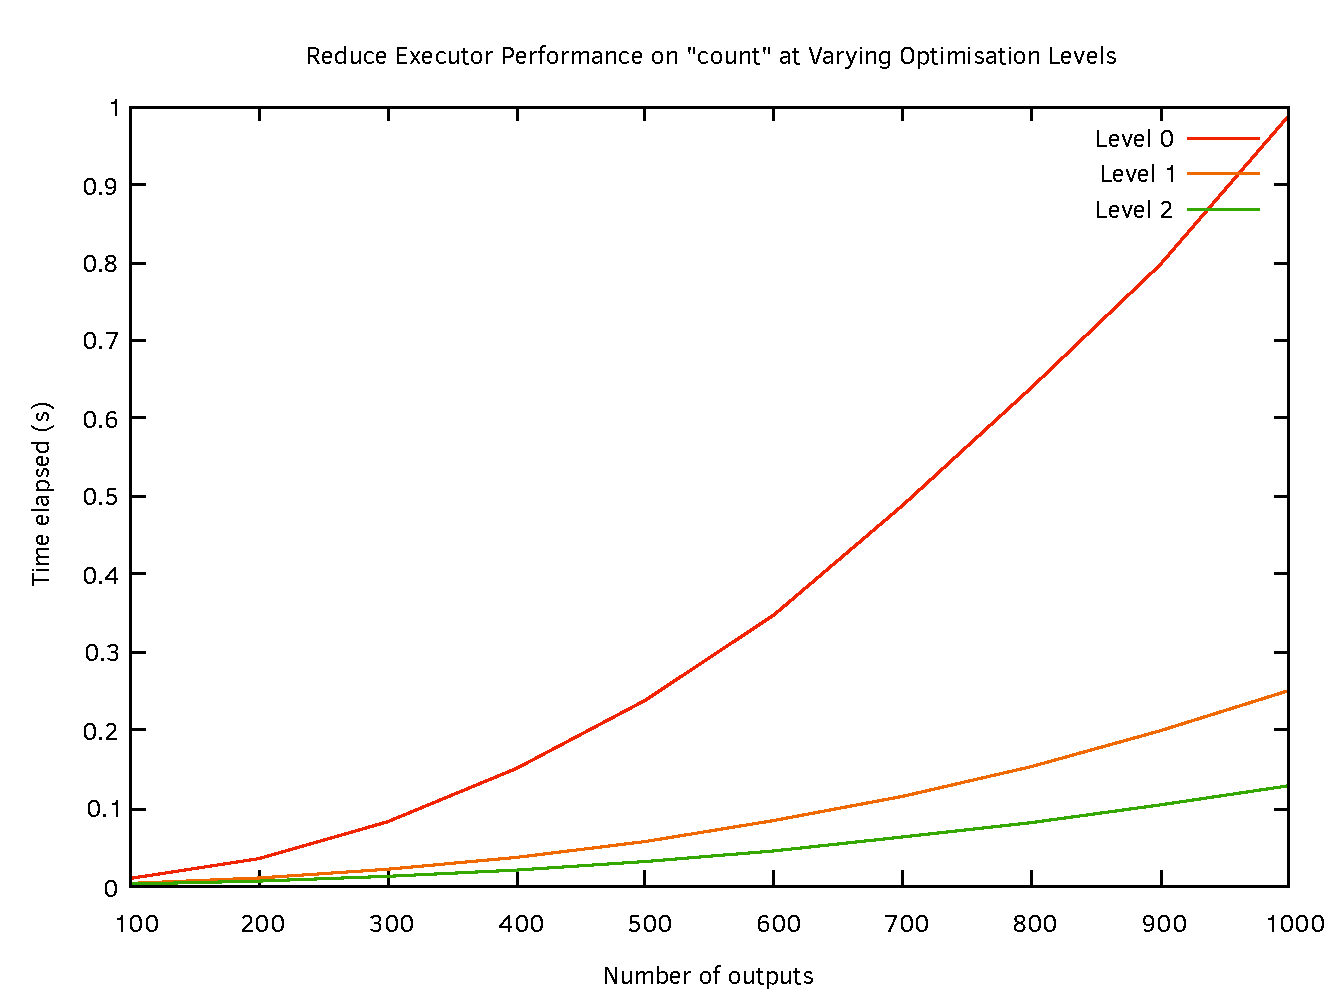
\includegraphics[width=\textwidth]{reduce_executor_fig_1}
    \caption{A chart demonstrating the effect of varying optimisations}
    \label{fig:reduce_executor_performance_on_count}
\end{figure}


Figure \ref{fig:reduce_executor_performance_on_count} shows the effects of the various optimisations on program performance. level 0 represents a baseline state without any optimisations.

\todo[inline]{Per instruction breakdown}

\todo[inline]{just rename to evaluation}
\todo[inline]{Put results here}
\todo[inline]{Merge results and evaluation?}

\todo[inline]{Talk about prelim results}
\todo[inline]{Talk about CPU profiling}